
\documentclass[journal]{IEEEtran}

\usepackage{epsfig, amsmath, amssymb, cite, booktabs, array, multirow}
\usepackage{dblfloatfix} 
\usepackage{arydshln}
\usepackage{mathtools}
\usepackage{mathrsfs}
\usepackage{boldline}
\usepackage{algorithm}
\usepackage{algorithmic}
% Use the postscript times font!
\usepackage{multirow}
\usepackage[normalem]{ulem}
\usepackage{graphicx}
\usepackage{enumitem}
% \usepackage{newfloat}
% \usepackage{listings}
% \usepackage{booktabs}
\usepackage{graphicx}
% \usepackage{multirow}
% \usepackage{amsmath}
% \usepackage{subfig}
\usepackage{makecell}
\usepackage{color}
\usepackage{subfigure}
\useunder{\uline}{\ul}{}
\makeatletter
\newcommand*{\rom}[1]{\expandafter\@slowromancap\romannumeral #1@}
\makeatother

% \usepackage{setspace}
% \onecolumn
% % \doublespacing%Allows double spacing with the \doublespacing command
% \setstretch{3.5}

%\usepackage[justification=centering]{caption}
%\usepackage[labelsep=period]{caption}
%\captionsetup[figure]{labelsep=period}

% correct bad hyphenation here
\hyphenation{op-tical net-works semi-conduc-tor}
\hyphenation{rep-re-sen-ta-tion}

\graphicspath{{./figure/}}

\newcommand\Tstrut{\rule{0pt}{2.6ex}}         % = `top' strut
\newcommand\Bstrut{\rule[-0.9ex]{0pt}{0pt}}   % = `bottom' strut


\begin{document}

\title{Oracle Teacher: Leveraging Target Information for Better Knowledge Distillation of CTC Models}
\author{Ji~Won~Yoon,~\IEEEmembership{Student Member,~IEEE}, 
Hyung~Yong~Kim,~\IEEEmembership{Student Member,~IEEE},
Hyeonseung~Lee,~\IEEEmembership{Student Member,~IEEE},
Sunghwan~Ahn,~\IEEEmembership{Student Member,~IEEE}, and Nam~Soo~Kim,~\IEEEmembership{Senior Member,~IEEE}

% \thanks{Manuscript received November 15 2021; revised -.}
\thanks{The authors are with the Department of Electrical and Computer Engineering and the Institute of New Media and Communications, Seoul National University, Seoul, Korea (e-mail: jwyoon@hi.snu.ac.kr, hykim@hi.snu.ac.kr, hslee@hi.snu.ac.kr, shahn@hi.snu.ac.kr, nkim@snu.ac.kr) (Corresponding author: Nam Soo Kim).}
}

% \thanks{This work has been submitted to the IEEE for possible publication. Copyright may be transferred without notice, after which this version may no longer be accessible.}}

\ifCLASSOPTIONpeerreview
\author{\IEEEauthorblockN{Ji~Won~Yoon,~\IEEEmembership{Student Member,~IEEE} and Nam~Soo~Kim,~\IEEEmembership{Senior Member,~IEEE}}
\IEEEauthorblockA{Department of Electrical and Computer Engineering and INMC,\\
Seoul National University \\
1 Gwanak-ro, Gwanak-gu, Seoul 08826, Korea \\
Tel: +82-2-880-8439 Fax: +82-2-880-8219 E-mail:
nkim@snu.ac.kr}} \fi

% The paper headers
\markboth{IEEE/ACM~TRANSACTIONS~ON~AUDIO,~SPEECH,~AND~LANGUAGE~PROCESSING,~Vol.~x, No.~x,~2022}%
{Shell \MakeLowercase{\textit{et al.}}: xxx}

% make the title area
\maketitle

% As a general rule, do not put math, special symbols or citations
% in the abstract or keywords.
\begin{abstract}
Knowledge distillation (KD), best known as an effective method for model compression, aims at transferring the knowledge of a bigger network (teacher) to a much smaller network (student). Conventional KD methods usually employ the teacher model trained in a supervised manner, where output labels are treated only as targets. Extending this supervised scheme further, we introduce a new type of teacher model for connectionist temporal classification (CTC)-based sequence models, namely Oracle Teacher, that leverages both the source inputs and the output labels as the teacher model's input. Since the Oracle Teacher learns a more accurate CTC alignment by referring to the target information, it can provide the student with more optimal guidance. One potential risk for the proposed approach is a trivial solution that the model's output directly copies the target input. Based on a many-to-one mapping property of the CTC algorithm, we present a training strategy that can effectively prevent the trivial solution and thus enables utilizing both source and target inputs for model training. Extensive experiments are conducted on two sequence learning tasks: speech recognition and scene text recognition. From the experimental results, we empirically show that the proposed model improves the students across these tasks while achieving a considerable speed-up in the teacher model's training time.
\end{abstract}

% Note that keywords are not normally used for peerreview papers.
\begin{IEEEkeywords}
Speech recognition, scene text recognition, connectionist temporal classification, knowledge distillation, teacher-student learning, transfer learning
\end{IEEEkeywords}

\IEEEpeerreviewmaketitle



\section{Introduction}

\IEEEPARstart{A}s deep neural networks bring a significant improvement in various fields such as speech recognition, computer vision, and natural language processing, they also become wider and deeper.
However, as models grow in size and complexity, high-performing neural network models become either computationally expensive or consume a large amount of memory, hindering their wide deployment in resource-limited scenarios.
To mitigate this computational burden, several techniques such as model pruning \cite{pruning1:scheme, pruning2:scheme}, quantization\cite{quantization:scheme}, and knowledge distillation \cite{bucila-et-al:scheme, hinton_kd-et-al:scheme} have been suggested.
Among these approaches, knowledge distillation (KD) is a popular compression scheme, which is the process of transferring knowledge from a deep and complex model (teacher) to a shallower and simpler model (student). 

Conventional KD methods typically share a common feature; they require a teacher model with high capacity that has been trained in a supervised manner, where the ground-truth labels are required as a target.
However, training the teacher from scratch can be costly since many of the current state-of-the-art (SOTA) models suffer from
excessive training time and difficult hyper-parameters tuning.
% \textcolor{blue}{To reproduce the results, some SOTA models require tremendous time and GPU resources.}
Thus, some existing approaches rely heavily on the pre-trained model, provided by other prior research, as the teacher to save the training time and resource cost.
Even though making full use of the provided pre-trained models is one important motivation of KD, this dependency might limit the flexibility of our consideration.
If we can train a better teacher model with fewer resources and training time, KD from various teachers will be possible on different tasks or databases.
% Even though making full use of the provided pre-trained models is one important motivation of KD, this dependency might limit the flexibility of our consideration on the task, model structure, dataset, etc.


We revisit the teacher model in KD from a different perspective.
% Imagine a real-world scenario; you are a teacher and have enough skills to teach your students to solve some problems. 
% Although you can solve various problems accurately on your own, it is often difficult to solve complex problems in an optimal way.
In a conventional KD scenario, there is no guarantee that the teacher can find the correct solution for every complicated problem in an optimal way, implying that the teacher model may provide suboptimal guidance for the student.
The key idea of our framework is to derive a more accurate problem-solving process by referring to the existing solutions so that the teacher can provide better guidance to the student.
On this basis, we introduce a new type of teacher for Connectionist Temporal Classification (CTC) \cite{graves-et-al:scheme}-based sequence models, namely Oracle Teacher.
The conventional teacher is typically built in a supervised manner whose goal is to predict the target output for a given source input data. 
In contrast, the proposed teacher model utilizes not only the source input but also the target value to estimate better CTC alignment.

% To the best of our knowledge, this is the first attempt of using the oracle input to train the teacher model.
% However, it is challenging to train the model using both the source inputs and the output labels as the model's input.
However, it may be somewhat confusing to understand what it means to train a model using both the source inputs and the output labels as the model's input.
Specifically, the Oracle Teacher is likely to heavily rely on the target input, i.e., the output label, while ignoring the embedding from the source input.
To overcome this problem, we propose a training scheme that uses the many-to-one mapping property of the CTC algorithm.
Since the relationship between the CTC alignment and the original target is many-to-one, 
we can prevent a trivial solution that the model's output directly copies the target input.
To the best of our knowledge, this is the first attempt of using the target input to improve the ability of the teacher model.
Utilizing the target input for training the teacher model brings several benefits for KD. Firstly, the proposed teacher model produces a more accurate CTC alignment by referring to the target information so that its knowledge can provide more optimal guidance to the student.
Secondly, the representation of the proposed teacher contains target-related embedding that can be supportive for student training. 
For example, the Oracle Teacher for automatic speech recognition (ASR) is trained to use both speech and text as the model's input during training.
Different from the typical ASR teachers that take only acoustic features into consideration, the Oracle Teacher performs a fusion of both acoustic (speech) and linguistic (text) features when generating the prediction.
Since unifying acoustic and linguistic representation learning generally enhances the performance of the speech processing \cite{acours_lin1,acours_lin2,acours_lin3,acours_lin4,acours_lin5}, the Oracle Teacher's representation, which considers not only the acoustic but also linguistic information, can be more effective for the ASR student.
Also, the Oracle Teacher can boost up the speed of the training since the target input is used as the guidance to reduce the candidate scope of the prediction. Compared to the conventional teacher models that require tremendous time and GPU resources, our framework dramatically reduces the computational cost required to train the teacher model.

% \begin{wrapfigure}{r}{.65\textwidth}
% \centering
%     \vspace{-3mm}
%     \hspace*{-3mm}%
% 	\includegraphics[height=2.5cm]{translation.jpg}
% % 	\vspace{-3mm}
%  	\caption{Visualized English-to-German translation example.}
% 	\label{translate}
% 	\vspace{-5mm}
% \end{wrapfigure}For example, Fig. \ref{translate} shows an example of machine translation (MT) task. Compared to the conventional teacher trained in the supervised manner, the proposed teacher model produces better translation prediction quality, implying that the Oracle Teacher can provide a more optimal guidance to the student.


Extensive experiments are conducted on two different sequence learning tasks: ASR and scene text recognition (STR). 
% The pre-trained model, which yields the state-of-the-art (SOTA) performance, is adopted as a conventional teacher for performance comparison in each task.
% Although there are many existing KD methods, we employ FitNets \cite{romero-et-al:scheme} as the basic KD technique to fairly compare the performance improvement of the student.
Empirically, we verify that the student distilled from the Oracle Teacher achieves better performance compared to the case when it is distilled from the other pre-trained models, which yield the high performance for each task.
Apart from performance, we also measure the computational cost for training teacher model and shows that a powerful teacher can be trained with a reduced computational burden via the proposed scheme.
% We also study the behavior of the Oracle Teacher and test if it has been correctly trained.

Our \textbf{main contributions} are summarized as follows:
\begin{enumerate}
    \item  Our paper introduces a new type of teacher for CTC-based sequence models, namely Oracle Teacher, that utilizes the output labels as an additional input for model training.
    The proposed teacher model can estimate a more accurate CTC alignment, providing more optimal guidance to the student.
    To the best of our knowledge, this is the first attempt of using the target input to improve the performance of a teacher model.
    \item Through extensive experiments on two sequence learning tasks, including ASR and STR, we verify the superiority of the Oracle Teacher compared to the conventional teacher models.
    Moreover, our framework dramatically reduces the computational cost of the teacher model in terms of the training time and required GPU resources.
    \item In a detailed case study and analysis, we validate why the proposed method can result in better KD performance than the conventional teacher and check if the Oracle Teacher is correctly trained while preventing the trivial solution.
    
\end{enumerate}

% The analysis of the experimental results is provided in Section \rom{6}. 
\section{Related work}
\label{2}
\subsection{Knowledge Distillation}
\label{2.1}
There has been a long line of research on KD, which aims at distilling knowledge from a big teacher model to a small student model. 
Bucila \textit{et al.} \cite{bucila-et-al:scheme} proposed a method to compress an ensemble of models into a single model without significant accuracy loss.
Later, Ba and Caruana \cite{dodeep:scheme} extended it to deep learning by using the logits of the teacher model.
Hinton \textit{et al.} \cite{hinton_kd-et-al:scheme} revived this idea under the name of KD that distills class probability by minimizing the Kullback-Leibler (KL)-divergence between the softmax outputs of the teacher and student.
In the case of the ASR task, the most frequently employed KD approach is to train a student with the teacher's prediction as a target, in conjunction with the ground truth.
For the conventional deep neural network (DNN)-hidden Markov model (HMM) hybrid systems, Li \textit{et al.} \cite{firstasr:scheme} first attempted to apply the teacher-student learning to a speech recognition task, and Wong \textit{et al.} \cite{seq:scheme} applied sequence-level KD to the acoustic model. Several researchers applied KD to improve the performance by minimizing the frame-level cross-entropy loss between the output distributions of the teacher and student \cite{blending:scheme,chebotar-et-al:scheme,watanabe-et-al:scheme,lu-et-al:scheme,fukuda-et-al:scheme}.
For end-to-end speech recognition, KD has been successfully applied to CTC models \cite{senior-et-al:scheme,takashima-et-al:scheme, takashima-et-al2:scheme, kurata2-et-al:scheme,kurata-et-al:scheme, tutornet:scheme} and attention-based encoder-decoder models \cite{compression:scheme, wer_error:scheme, entropy:scheme, tutornet:scheme}.
However, as reported in previous KD studies \cite{senior-et-al:scheme,takashima-et-al:scheme, takashima-et-al2:scheme, tutornet:scheme}, simply applying the frame-level CE to the CTC-based model can worsen the performance compared to the baseline.
To cover this problem, Kurata and Audhkhasi \cite{kurata-et-al:scheme, kurata2-et-al:scheme} proposed KD approaches, where the CTC-based student can be trained using the frame-wise alignment of the teacher.
Takashima \textit{et al.} \cite{takashima-et-al:scheme,takashima-et-al2:scheme} explored sequence-level KD methods for training CTC models.
Yoon \textit{et al.} \cite{tutornet:scheme} suggested that $l_{2}$ loss is more suitable than the conventional KL-divergence to distill frame-level posterior in the CTC framework.


The hidden representation from the teacher also has been proven to hold additional knowledge that can contribute to improving the student's performance.
Recently, some KD methods \cite{romero-et-al:scheme,at:scheme,fsp:scheme,jacobian:scheme,factor:scheme, boundary:scheme, relation:scheme, showanddistill:scheme}, particularly in computer vision, were proposed to minimize the mean squared error (MSE) between the representation-level knowledge of the two models.
They address how to extract a better knowledge from the teacher model and transfer it to the student.
Yoon \textit{et al.} \cite{tutornet:scheme} first attempted to transfer the the hidden representation across different structured neural networks for end-to-end speech recognition while using frame weighting that reflects which frames are important for KD.
Recently, several KD approaches \cite{distillhubert:scheme, lighthubert:scheme,fithubert} suggested using the hidden representation-level knowledge to improve the self-supervised speech representation learning-based models, like Hidden-Unit BERT (HuBERT).
% \subsection{Sequence Model}
% \label{2.1}
% End-to-end sequence models can be roughly classified into two groups based on the network architecture and loss type: 1) Connectionist Temporal Classification (CTC) \cite{graves-et-al:scheme} models and 2) Attention-based Encoder-Decoder (AED),
% e.g., Listen-Attend-Spell \cite{las:scheme,chorowski-et-al:scheme} or Transformer \cite{transformer:scheme}.
\begin{figure}[t]
\centering
	\includegraphics[height=10cm]{overview3.png}
	\caption{Overview of the Oracle Teacher. The proposed teacher model mainly consists of three components: the SourceNet, the encoder, and the decoder. Different from the conventional teacher, the target $y$ is used as the additional input to the model. Note that the Oracle Teacher is a non-autoregressive model where the look-ahead mask is not included in the decoder. The architecture selection of the SourceNet depends on the task we are interested in. When the main task is ASR. the SourceNet corresponds to an acoustic model part of the conventional ASR model. In our experiment for ASR, the SourceNet is based on the architecture of Japser \cite{jasper:scheme}. For STR, we apply the CRNN \cite{crnn:scheme} as the SourceNet.}
	\label{oracle_arc}
\end{figure}

\begin{figure}[t]
    \centering
    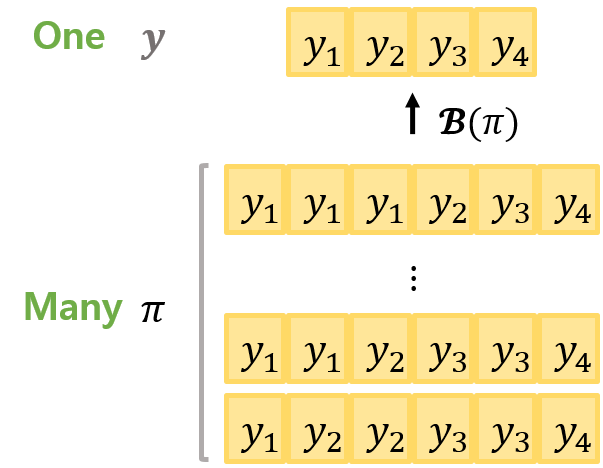
\includegraphics[height=3.1cm]{manytoone.png}
    \caption{The relationship between the CTC alignment $\pi$ and the target input $y$. A many-to-one mapping function $\mathcal{B}$ converts the alignment sequence $\pi$ into the final output sequence $y$.}
    \label{CTC_MANY}
\end{figure}

\subsection{Connectionist Temporal Classification}
\label{2.2}
Generally, an end-to-end sequence model directly converts a sequence of input features $x_{1:T}$ into a sequence of target labels $y_{1:L}$ where $y_{l} \in \mathcal{I}$ with $\mathcal{I}$ being the set of labels. $T$ and $L$ are respectively the length of $x=x_{1:T}$ and $y=y_{1:L}$. 
To cope with the mapping problem when the two sequences have different lengths, the Connectionist Temporal Classification (CTC) framework \cite{graves-et-al:scheme} introduces~``blank" label and allows the repetition of each label to force the output and input sequences to have the same length. A CTC alignment $\pi_{1:T}$ is a sequence of initial output labels, as every input $x_{t}$ is mapped to a certain label $\pi_{t} \in \mathcal{I'}$ where $\mathcal{I'} = \mathcal{I} \cup \{blank\}$. A mapping function $\mathcal{B}$, which is defined as $y = \mathcal{B}(\pi)$, maps the alignment sequence $\pi$ into the final output sequence $y$ after merging consecutive repeated characters and removing blank labels. 
% For example, two alignment sequences $\{\varepsilon, c, c, c, \varepsilon, a, \varepsilon, \varepsilon, t, t, \varepsilon\}$ and $\{c, c, \varepsilon, \varepsilon, a, a, \varepsilon, \varepsilon, \varepsilon, \varepsilon, t\}$ (using ~`$\varepsilon$' to denote blank label) correspond to the same sequence $\{c, a, t\}$ through the mapping function $\mathcal{B}$. 
% The alignment between the input $x$ and the target output $y$ is not explicitly required in CTC training.
The conditional probability of the target sequence $y$ given the input sequence $x$ is defined as
\begin{equation}
   P(y \vert x) = \sum_{\pi \in \mathcal{B}^{-1}(y)} P(\pi \vert x).
   \label{ctc}
\end{equation}
where $\mathcal{B}^{-1}$ denotes the inverse mapping and returns all possible alignment sequences compatible with $y$.
% Since many different intermediate sequences can be mapped into the same target sequence, the conditional probability is defined as the sum of probabilities of all possible intermediate sequences. 
Given a target label sequence $y$, the loss function $\mathcal{L}_{CTC}$ is defined as:
%
\begin{align}
  \mathcal{L}_{CTC} = - \log P(y \vert x) .
\end{align}%

% \subsection{Attention-Based Sequence Model}
% \label{2.3}
% An alternative approach to the end-to-end mapping between $x_{1:T}$ and $y_{1:L}$ is to use the attention-based model, e.g., Listen-Attend-Spell \cite{las:scheme,chorowski-et-al:scheme} or Transformer \cite{transformer:scheme}. 
% Conditioned on previously generated output tokens and the full input sequence, the model factorizes the joint target sequence probability into a product of individual time steps. It is trained by minimizing the token-level cross-entropy (CE) loss between $y$ and the decoder predicted distributions.

\section{Oracle Teacher}
This section introduces how to design the Oracle teacher that utilizes the output labels as an additional input.
As shown in Fig. \ref{oracle_arc}, we let the Oracle Teacher model learn a function from the source $x$ and the target $y$ inputs to the CTC alignment $\pi$.

\subsection{Oracle Teacher Training}
Let $x=x_{1:T}=\{x_{1},...,x_{T}\}$ be an input sequence of length $T$, and $y=y_{1:L}=\{y_{1},...,y_{L}\}$ be a target sequence of length $L$.
As mentioned in Section \ref{2.2},  the CTC algorithm employs the intermediate CTC alignment $\pi=\pi_{1:T}=\{\pi_{1},...,\pi_{T}\}$ to align variable-length input and output sequences.
As shown in Fig. \ref{CTC_MANY}, the relationship between the alignment $\pi$ and the target input $y$ is many-to-one via the mapping $\mathcal{B}$, and this many-to-one setting is the key to training the Oracle Teacher.
Intuitively, predicting the CTC alignment $\pi$ (many) from the target input $y$ (one) should be difficult since many possible paths are compatible with $y$.
Therefore, the proposed model can be trained to use the embeddings of both $x$ and $y$ while preventing a trivial solution where the model's output simply copies the input $y$.
The Oracle Teacher can effectively estimate the most probable CTC alignment $\pi$ since the target input $y$ is used as guidance to reduce the candidate scope of $\pi$.
The Oracle Teacher learns the parameters $\theta$ to minimize the following training loss:
\begin{equation}
\label{oracle}
\mathcal{L}_{train} = -\log\sum_{\pi \in \mathcal{B}^{-1}(y)}P(\pi|x,y;\theta)
\end{equation}
where $\mathcal{B}$ is the many-to-one mapping function in (\ref{ctc}) that maps the latent alignment $\pi_{1:T}$ into the target $y_{1:L}$.

% As shown in Fig. \ref{CTC_MANY}, the relationship between the CTC alignment $\pi$ and the target input $y$ is many-to-one via the mapping $\mathcal{B}$, and this many-to-one setting is the key to training the Oracle Teacher.
% Intuitively, predicting the CTC alignment $\pi$ (many) from the target input $y$ (one) should be difficult since many possible paths are compatible with $y$.
% Therefore, the proposed model can be trained to use the embeddings of both $x$ and $y$ while preventing a trivial solution where the model's output simply copies the input $y$.


% \subsection{CE as Objective}
% \label{3.2.2}
% Unlike CTC, the many-to-one mapping $\mathcal{B}$ and the latent alignment $\pi$ do not exist in the CE-based model, resulting in a one-to-one correspondence between $\pi$ and $y$, i.e., $\pi=y$.
% Therefore, we use random masking to relax the one-to-one constraint into the many-to-one relationship.
% Inspired by BERT \cite{devlin-et-al:schoeme}, we randomly mask a set of tokens in the input $y$. Masked target $\tilde{y}$ is given as
% \begin{align}
% \label{mask}
%    \tilde{y} \sim Mask(y, \lambda)
% \end{align}%

% where $Mask(\cdot)$ denotes the mapping that masks the tokens of $y$ with the probability of $\lambda$.
% Instead of $y_{1:L}$, the masked target $\tilde{y}_{1:L}$ is fed to the Oracle Teacher to predict $\pi_{1:L}$, similar to the masked language modelling in BERT.

% As shown in Fig. \ref{CE_MANY}, assuming that the target of the CE-based Oracle Teacher is $\pi_{1:4}=y_{1:4}=\{y_{1}, y_{2}, y_{3}, y_{4}\}$ given the masked input $\tilde{y}_{1:4}=\{y_{1}, [mask],[mask],y_{4}\}$. 
% Due to $\pi=y$, Equation (\ref{mask}) can be considered as $\tilde{y}\sim Mask(z, \lambda)$.
% Since predicting the complete target $\pi$ (many) only from the incomplete target input $\tilde{y}$ (one) is impossible, the Oracle Teacher is trained to use both $x$ and $y$ as the model's input in training, preventing the trivial solution.
% In the CE framework, $Mask(\cdot)$ is used as the many-to-one mapping, and the relationship between the target $\pi$ and the masked target input $\tilde{y}$ can be regarded as many-to-one.jwyo
% Therefore, CE-based Oracle Teacher is trained to minimize the following objective function:

% \begin{equation}
% \mathcal{L}_{train} = -\log P(\pi|x,\tilde{y};\theta).
% \end{equation}
% where $\pi=y$. The proposed scheme can easily find the global optimum solution with the guidance of $\tilde{y}$ where $\tilde{y}=Mask(\pi)$.


\subsection{Knowledge Distillation with Oracle Teacher} 
\label{oracle_kd_section}
We can interpret KD framework from a different perspective by applying the additional target input.
Given a source $x$, the student model learns the parameter $\phi$ to maximize the following conditional probability:
\begin{align}
\label{kl}
  \log P(y|x;\phi) & = \log\int_{\pi}P(y,\pi|x;\phi)\,d\pi  \nonumber \\
    & = \log\int_{\pi}P(y,\pi|x;\phi)\frac{P(\pi|x,y;\theta)}{P(\pi|x,y;\theta)}\,d\pi \nonumber \\
  & = \log\int_{\pi}\delta(y-\mathcal{B}(\pi))P(\pi|x;\phi)\frac{P(\pi|x,y;\theta)}{P(\pi|x,y;\theta)}\,d\pi \nonumber \\
 & = \log\int_{\pi\in\mathcal{B}^{-1}(y)}P(\pi|x,y;\theta)\frac{P(\pi|x;\phi)}{P(\pi|x,y;\theta)}\,d\pi \nonumber \\
  & \geq \int_{\pi\in\mathcal{B}^{-1}(y)}P(\pi|x,y;\theta)\log\frac{P(\pi|x;\phi)}{P(\pi|x,y;\theta)}\,d\pi  \nonumber \\
  & = - D_{KL}(\underbrace{P(\pi|x,y;\theta)}_{\text{Oracle Teacher}} \Vert \underbrace{P(\pi|x;\phi)}_{\text{Student}}) 
\end{align}%
where the inequality follows from Jensen’s inequality, $\mathcal{B}$ represents the mapping function in (\ref{oracle}), and $D_{KL}$ denotes the KL-divergence. 
In our framework, $P(\pi|x,y;\theta)$ and $P(\pi|x;\phi)$ correspond to the alignment probability derived from the Oracle Teacher and the student, respectively.
By minimizing the KL-divergence between the Oracle Teacher and the student, we can maximize the conditional probability of the student model $P(y|x;\phi)$.

\begin{figure}[t]
\centering
    % \vspace{-3mm}
    % \hspace*{-5mm}%
	\includegraphics[height=4.7cm]{kd.png}
	% \vspace{-3mm}
	\caption{KD procedure with the Oracle Teacher.}
	\label{oracle_kd}
	% \vspace{-3mm}
\end{figure}
Directly optimizing the KL-divergence in (\ref{kl}) is intractable because the KL divergence involves the integral that is difficult to calculate.
To sidestep this problem, we can minimize the CE between the softmax outputs of the Oracle Teacher and the student.
However, as reported in previous KD studies \cite{senior-et-al:scheme,takashima-et-al:scheme, takashima-et-al2:scheme}, simply applying the frame-level CE to the CTC-based model can worsen the performance compared to the baseline trained only with the ground truth.
Instead, we adopt FitNets \cite{romero-et-al:scheme} as the basic KD technique, which considers the hidden representation for distillation, and there are two reasons for this choice: (1) In the CTC framework, transferring the hidden representation is much more effective than the softmax-level KD approach \cite{tutornet:scheme}; (2) Recent KD approaches for sequence learning \cite{tutornet:scheme,distillhubert:scheme,fithubert} are based on the Fitnets.

As depicted in Fig. \ref{oracle_kd}, $w_{tea}$ and $w_{stu}$ respectively denote the hidden representation obtained from the last layer of the teacher and student models.
Since usually the hidden layer dimensions of $w_{tea}$ and $w_{stu}$ are different, we apply a fully connected layer $g$ to bridge the dimension mismatch. The process of KD initializes the student by minimizing the distance between hidden representation of the teacher model $w_{tea}$ and student model $w_{stu}$.
The objective for KD is given by
\begin{align}
\label{hidden}
   \mathcal{L}_{KD}(w_{stu}, w_{tea}) =\Vert{w_{tea}-g(w_{stu})}\Vert_2^2.
\end{align}%

\subsection{Model Structure}
\label{oracle_model_structure}
The Oracle Teacher mainly consists of three components: 1) an encoder to encode the target input, 2) a SourceNet to extract the features from the source input data, and 3) a decoder to predict the CTC alignment.
Its architecture follows the encoder-decoder structure of the Transformer \cite{transformer:scheme}, which allows the model to attend to related target information when making a prediction.
Note that the Oracle Teacher is a non-autoregressive model where the look-ahead mask is not included in the decoder.
% Note that the decoder forms the queries from the SourceNet and key-value pairs from the  encoder.
In Fig. \ref{oracle_arc}, we illustrate the schematics of the Oracle Teacher model which can also be
summarized as follows:
\begin{align}
\label{oracle_align}
  & h^{S}=\text{SourceNet}(x;\theta_{S}), \\
  & h^{E}=\text{Encoder}(y;\theta_{E}), \\
  & P(\pi|x,y) \sim \text{Decoder}(h^{E}, h^{S};\theta_{D}). 
 \end{align}
% where $h^{S}$ and $h^{E}$ denote the representation from the SourceNet and the encoder, respectively.
Compared to the vanilla Transformer, the main architectural difference lies in the cross attention. The encoder takes inputs from the whole target $y$, and its resulting vectors $h^{E}$ are treated as key-value pairs of the cross attention.
In addition, we do not employ a look-ahead mask, which is used in the vanilla Transformer to mask the future tokens, in the multi-head attention layer of the decoder.

\subsubsection{SourceNet}
The SourceNet converts the source input $x$ into high-level representations $h^{S}$.
Since $h^{S}$ serves as query for the decoder, the length of the decoder output has the same length as $h^{S}$.
The architecture of the SourceNet depends on the task we are interested in.
When the main task is ASR. the SourceNet corresponds to an acoustic model part of the conventional ASR model.
In our experiments, we apply CTC-based Jasper \cite{jasper:scheme} architecture as the SourceNet, and consequently $|h^{S}|\geq|y|$. 
In the case of the STR task, we adopt the architecture of the CRNN \cite{crnn:scheme} for the SourceNet.
% In the case of MT, the SourceNet is based on the vanilla Transformer \cite{transformer:scheme}, and then $|h^{S}|=|y|$ during the training. 
% Note that $x$ and $h^{S}$ do not necessarily match in their lengths.
% For instance, in the MT task, the SourceNet follows the original Transformer architecture, where its internal decoder outputs $h^{S}$ using a teacher-forcing manner.
% As the output sequence length in the Transformer is possibly different from the length of the source sequence, $x$ and $h^{S}$ can have different lengths.
\subsubsection{Encoder}
In the encoder, we adopt the same structure as the encoder of the original Transformer. 
The self-attention captures dependencies between different positions in $y$ and outputs intermediate representations $h^{E}$.
% In the case of CE training, the masked target $\tilde{y}$ is fed to the encoder instead of $y$.
\subsubsection{Decoder}
The representations $h^{S}$ and $h^{E}$ are fed into the decoder, which follows the architecture of the conventional Transformer decoder.
The self-attention layer, the first attention layer of the decoder, takes the representations $h^{S}$ as the input.
Then, the output serves as queries for the cross attention, whose key-value pairs are the representations $h^{E}$.
The cross attention allows the decoder to look into the relevant target information when producing the prediction.
Note that the look-ahead mask is not included in the decoder.
Different from the autoregressive model that only uses the past output tokens in producing the results, the Oracle Teacher can utilize more global output features when predicting the output.

% When swapping the inputs of the encoder and the decoder, the structure is similar to the original Transformer, not the Oracle Teacher.
% Then, the model's output length is equal to $L$, which is the length of the target $y$.
In the proposed framework, the representation of the source $x$ corresponds to the queries for the cross-attention.
This is because, for KD, the length of the decoder output (= the length of the query $h^S$) should have the same length ($T$) as the student's output, which is determined by the source $x$.
If the decoder output has a different length from that of the student's output, the Oracle Teacher cannot transfer the knowledge to the student.



\section{Experimental Settings}
\subsection{Datasets and Baselines}
\subsubsection{Speech Recogniton}
For ASR, we evaluated the performance of the models on LibriSpeech \cite{librispeech:scheme}. In the training phase, ~``train-clean-100",~``train-clean-360", and~``train-other-500" were used. For evaluation, ~``dev-clean",~``dev-other",~``test-clean", and ~``test-other" were applied. 
We adopted the current high-performing models for the conventional teacher in each task. In the case of ASR, we applied pre-trained Jasper Dense Residual (Jasper DR) \cite{jasper:scheme}, which consists of 54 convolutional layers.
Recent ASR studies \cite{tutornet:scheme, asr1, asr2, asr3} utilized Jasper DR as the baseline.
According to the previous study \cite{jasper:scheme}, Jasper DR produces word error rate (WER) 2.62 \% with strong Transformer-XL \cite{transformer-xl} LM, still SOTA performance on LibriSpeech.
As for the ASR student model, we used Jasper Mini, composed of 33 depthwise separable 1D convolutional layers.
The Oracle Teacher had the SourceNet with 8 convolutional layers, and both the encoder and decoder consisted of 2 layers.
% We evaluated the MT models on IWSLT 2016 datasets for English-to-German (En-De), German-to-English (De-En), English-to-French (En-Fr), and French-to-English (Fr-En) translation tasks. 
% We used tst2013 as the validation set, and tst2013 and tst2014 were applied as test sets.
\begin{table*}[t]
% \renewcommand{\tabcolsep}{3.5pt}
\centering
\caption{WER (\%) performance comparison across CTC-based ASR models on LibriSpeech. The best result of the student is in bold.}{% 
{\fontsize{7.3}{8.76}\selectfont
% \vspace{-2mm}
\label{sr_result}
\begin{tabular}{|c|c|c|c|c|c|c|c|c|c|}
\hline
\multirow{3}{*}{\makecell{ASR baseline\\model}} &\multirow{3}{*}{Params.}& \multicolumn{4}{c|}{w/o LM}  & \multicolumn{4}{c|}{w/ LM}                                       \\ \cline{3-10}
             &        & \multicolumn{2}{c|}{dev} &\multicolumn{2}{c|}{test}& \multicolumn{2}{c|}{dev} &\multicolumn{2}{c|}{test}           \\\cline{3-10}
             &        & clean         & other          & clean         & other          & clean         & other          & clean         & other          \\
\hline
Jasper DR \cite{jasper:scheme}& 333 M & 3.61 & 11.37 & 3.77 & 11.08 & 2.99 & 9.40 & 3.62 & 9.33\\
Jasper Mini & 8 M & 8.66          & 23.28          & 8.85          & 24.26          & 4.78          & 15.14          & 5.15          & 15.77          \\
\hline
\hline
\multirow{3}{*}{Student}&\multirow{3}{*}{Teacher} & \multicolumn{4}{c|}{w/o LM}                                      & \multicolumn{4}{c|}{w/ LM}                                       \\\cline{3-10}
    &        & \multicolumn{2}{c|}{dev}&\multicolumn{2}{c|}{test}& \multicolumn{2}{c|}{dev}&\multicolumn{2}{c|}{test}\\\cline{3-10}
   &         & clean         & other          & clean         & other          & clean         & other          & clean         &other          \\
\hline
\multirow{4}{*}{Jasper Mini}&None             & 8.66          & 23.28          & 8.85          & 24.26          & 4.78          & 15.14          & 5.15          & 15.77          \\
&Jasper DR \cite{jasper:scheme}                & 7.05          & 19.41          & 7.03          & 20.41          & 4.80          & 14.32          & 5.00          & 14.99          \\
&\textbf{Oracle Teacher (ours)}& \textbf{6.64} & \textbf{18.91} & \textbf{6.67} & \textbf{19.82} & \textbf{4.65} & \textbf{14.31} & \textbf{4.90} & \textbf{14.65} \\
&Oracle Teacher w/o target   & 7.22          & 20.39              & 7.32             & 21.10              & 4.72            & 14.67              & 4.91             & 15.15       \\     
\hline
\end{tabular}}}
\end{table*}

\subsubsection{Scene Text Recognition}
We evaluated STR models on seven benchmark datasets\footnote{We applied the datasets used in the comparative study conducted by Baek \textit{et al.} \cite{clova:scheme}.}: Street View Text (SVT) \cite{svt:scheme}, SVT Perspective (SVTP) \cite{svtp:scheme}, IIIT5K-Words (IIIT) \cite{iiit:scheme}, CUTE80 (CT) \cite{cute:scheme}, ICDAR03 (IC03) \cite{ic03:scheme}, ICDAR13 (IC13) \cite{ic13:scheme}, and ICDAR15 (IC15) \cite{ic15:scheme}.
For validation, IC13, IC15, IIIT, and SVT were applied. 
As training datasets, we used the two most popular datasets: MJSynth \cite{mj:scheme} and SynthText \cite{st:scheme}. 
We adopted Rosetta \cite{rosetta:scheme} and STAR-Net \cite{starnet:scheme}, considered as the benchmarking SOTA models in recent researches \cite{textocr, ocr2}.
In the case of the student model, CRNN \cite{crnn:scheme} was adopted with a thin-plate spline (TPS), which normalizes curved and perspective texts into a standardized view.
The SourceNet followed the TPS-CRNN structure, and both the encoder and decoder used 1 layer.
% For MT, we adopted the vanilla Transformer \cite{transformer:scheme}, which had 6 layers in both encoder and decoder based on the latest configurations of ESPnet \cite{espnet:scheme} toolkit. 
% In the case of the IWSLT dataset, many recent studies \cite{iwslt1,iwslt2,iwslt3} used a similar model setting for the baseline due to its promising performance.
% MT student baseline was built based on the Transformer. 
% For ease of comparison, we let Transformer$_{tea}$ and Transformer$_{stu}$ denote the conventional teacher and the student, respectively.
% For Transformer$_{stu}$, we used the vanilla Transformer with 3 encoder layers and 3 decoder layers.

% For ASR task, the Oracle Teacher had the SourceNet with 8 convolutional layers, and both the encoder and decoder consist of 2 layers.
% In the case of STR, the SourceNet followed the TPS-CRNN structure, and both the encoder and decoder used 1 layer.
% For MT, the Oracle Teacher includes the SourceNet, 1 encoder layer, and 1 decoder layer.
% The architecture of the SourceNet had 3 Transformer encoder and decoder layers.





\subsection{Implementation Details}
\subsubsection{Speech Recognition}
For the LibriSpeech dataset, We used the OpenSeq2Seq \cite{openseq2seq} toolkit for the implementation. ASR models were based on the character-level CTC models. 
The character set had 29 labels. In the case of Jasper DR, we used the pre-trained model provided by the OpenSeq2Seq toolkit. The student model was run on three Titan V GPUs, each with 12GB of memory.
We used a NovoGrad optimizer \cite{ginsburg-et-al:scheme} whose initial learning rate started from 0.02 with a weight decay of 0.001. 
For KD, the student was initially trained with FitNets \cite{romero-et-al:scheme} loss for 5 epochs.
After initialization, 50 epochs were spent on CTC training.
In addition, we trained the Oracle Teacher for 30 epochs on a single Titan V GPU using Noam learning rate scheduler with 4000 steps of warmup and a learning rate of 1.5. 
When applying beam-search decoding with language model (LM), we used KenLM \cite{Heafield2011KenLMFA} for 4-gram LM, where the LM weight, the word insertion weight, and the beam width were experimentally set to 2.0, 1.5, and 512, respectively.
For the Mandarin ASR dataset, the character set had a total of 5207 labels. Pre-trained Jasper DR, which was used as the conventional teacher, was provided by the NeMo \cite{nemo:scheme} toolkit. The student was trained in an identical way to LibriSpeech, but the initial learning rate was set to 0.005.
Instead of WER, we measured the character error rate (CER) since a single character often represents a word for Mandarin. 

\subsubsection{Scene Text Recognition}
When training the STR models, our experiments were conducted using the official implementation provided by Baek \textit{et al.}\footnote{https://github.com/clovaai/deep-text-recognition-benchmark} \cite{clova:scheme}. 
STR models were based on the character-level CTC models.
The character set had a total of 37 labels.
All STR models, including the Oracle Teacher, were trained for 300k iterations on a single Titan V GPU (12GB) in the CTC framework.
We employed the AdaDelta optimizer \cite{adadelta:scheme} with a decay rate of 0.95, and the initial learning rate was 1.0.
In FitNets \cite{romero-et-al:scheme} training, we trained 300k iterations for the student.



\begin{table*}[t]
\centering
\caption{CER (\%) on AISHELL-2 when greedy decoding was applied. The best result of the student is in bold.}{% 
{\fontsize{7.3}{8.76}\selectfont
\label{sr_result_aishell}
\begin{tabular}{|c|c|c|c|c|c|c|c|}
\hline
\multirow{2}{*}{\makecell{ASR baseline\\model} } & \multirow{2}{*}{Params.} &  \multicolumn{3}{c|}{dev} & \multicolumn{3}{c|}{test}\\ \cline{3-8}
  &          & iOS & Android & Mic & iOS & Android & Mic\\
\hline
Jasper DR \cite{jasper:scheme} & 338 M & 9.69 & 11.48 & 12.23 & 9.37 & 10.84 & 11.84\\
Jasper Mini& 14 M & 11.77 & 14.23 & 15.03 & 11.38 & 12.71 & 14.27 \\
\hline
\hline
\multirow{2}{*}{Student} & \multirow{2}{*}{Teacher} &  \multicolumn{3}{c|}{dev} & \multicolumn{3}{c|}{test}\\ \cline{3-8}
  &          & iOS & Android & Mic & iOS & Android & Mic\\
\hline
\multirow{4}{*}{Jasper Mini} &None & 11.77 & 14.23 & 15.03 & 11.38 & 12.71 & 14.27\\
&Jasper DR \cite{jasper:scheme}                 & 10.70&12.78&13.66&10.12&11.31&12.60 \\
&\textbf{Oracle Teacher (ours)}& \textbf{9.74}&\textbf{11.49}&\textbf{12.31}&\textbf{9.27}&\textbf{10.36}&\textbf{11.99}\\
&Oracle Teacher w/o target   & 10.45&12.42&13.13&9.76&10.92&12.19\\      
\hline
\end{tabular}}
}
% \caption{Experimental results on the ASR task.}
% \label{sr_ex}
\end{table*}
\section{Experimental Results}
In the subsequent part of this paper, $A$ $\rightarrow$ $B$ means that teacher model $A$ transfers knowledge to the student model $B$.
As mentioned in Section \ref{oracle_kd_section}, we employed FitNets \cite{romero-et-al:scheme} as the basic KD technique. 

% ASR and STR models were CTC-based models. MT models were trained with CE. 
% Note that we employed FitNets \cite{romero-et-al:scheme} as the baseline KD technique.
% Section \rom{5}-A covers performance comparison of the Oracle Teacher with other conventional teachers, and Section \rom{5}-B presents a detailed computational cost analysis (the number of parameters, training time, etc.) of the teacher models. Then, Section \rom{5}-C provides the attention visualization of the Oracle Teacher.

\subsection{Main Results: Performance Comparison}
Since the Oracle Teacher is the teacher model for KD, not the baseline model performing the learning task, the evaluation results of the Oracle Teacher itself are not described in this section. Note that the model size and the performance of the Oracle Teacher will be additionally discussed in Section \ref{computational cost section} and \ref{per_oracle}.
\begin{table*}[t]
% \renewcommand{\tabcolsep}{3.5pt}
\centering
\caption{Performance of CTC-based STR models. The best result of the student is in bold.}{%
{\fontsize{7.3}{8.76}\selectfont
\centering
% \vspace{-2mm}
\begin{tabular}{|c|c|c|c|c|c|c|c|c|c|c|c|c|}
\hline
\makecell{STR baseline\\model} & Params. & \makecell{IIIT\\3000}     & SVT             & \makecell{IC03\\860}         & \makecell{IC13\\857}        &\makecell{IC13\\1015}       & \makecell{IC15\\1811}       & \makecell{IC15\\2077}       & SVTP            & CT          & \makecell{Total\\accuracy}  \\
\hline
Rosetta \cite{rosetta:scheme} & 46 M & 85.53 & 84.85 &94.19  &91.95 &90.74 &73.22 &70.55 &76.12 &68.99 &82.45 \\
Star-Net \cite{starnet:scheme} & 49 M & 85.50 & 85.47 & 93.84  &92.77 & 91.92 &72.50 &69.77 &73.80 &70.38 &82.24\\
CRNN \cite{crnn:scheme}  & 10 M  & 83.87          & 80.37          & 93.02            & 90.43          & 89.46          & 70.07          & 67.53          & 72.09          & 65.51          & 80.10          \\
 \hline
 \hline
  Student&Teacher                   & \makecell{IIIT\\3000}     & SVT             & \makecell{IC03\\860}            & \makecell{IC13\\857}        &\makecell{IC13\\1015}       & \makecell{IC15\\1811}       & \makecell{IC15\\2077}       & SVTP            & CT          & \makecell{Total\\accuracy}  \\
\hline
\multirow{5}{*}{CRNN \cite{crnn:scheme}} & None    & 83.87          & 80.37          & 93.02              & 90.43          & 89.46          & 70.07          & 67.53          & 72.09          & 65.51          & 80.10          \\
&Rosetta \cite{rosetta:scheme} &   84.70          & 83.46          & 92.91                 & 91.02          & 90.15          & 71.89          & 69.20          & 71.16          & 65.85          & 81.04          \\
&Star-Net \cite{starnet:scheme} &   85.20          & 84.39          & 93.49         & \textbf{91.60} & \textbf{90.74} & 72.45          & 69.77          & 72.25          & 70.04          & 81.77          \\
&\textbf{Oracle Teacher (ours)}& \textbf{85.77} & \textbf{84.54} & \textbf{93.61}         & 91.48          & 90.54          & \textbf{73.11} & \textbf{70.40} & \textbf{74.26} & \textbf{70.38} & \textbf{82.21} \\
&Oracle Teacher w/o target& 85.40 & 82.84 & 93.02 & 90.78 & 89.75 & 71.73 & 69.04 & 72.71 & 68.99 & 81.30 \\
\hline
\end{tabular}%
\label{str_results}
}}
% \vspace{-5mm}
\end{table*}



\subsubsection{Speech Recognition} 
The results for LibriSpeech are shown in Table \ref{sr_result}.
We measured WER to quantify the performance.
% We adopted Jasper DR as the conventional teacher and Jasper Mini as the student.
The best performance was achieved when training the student with the Oracle Teacher.
In addition, to further check the effectiveness of the target input $y$, which is used as the additional input of the Oracle Teacher, we applied an incomplete Oracle Teacher model, called Oracle Teacher w/o target.
In Oracle Teacher w/o target, zero arrays were treated as the additional input instead of the target input $y$ during training and inference phases.
Since the Oracle Teacher w/o target only consumed the source input, its architecture was similar to that of the conventional CTC model.
When applying the Oracle Teacher w/o target, the distilled student achieved improvement over the baseline student, which indicates that the knowledge of the SourceNet contributed to improving the performance of the student.
However, their performances were worse than the Oracle Teacher $\rightarrow$ Jasper Mini in all configurations, implying that the oracle guidance helped the Oracle Teacher extract a more supportive knowledge for the student.

As presented in Table \ref{sr_result_aishell}, we can confirm that the Oracle Teacher still works well with KD on the Mandarin dataset.
Interestingly, when the Oracle Teacher was applied, the distilled student (CER: 9.74 \% on dev-iOS) performed similarly to the pre-trained Jasper DR (CER: 9.69 \% on dev-iOS), notwithstanding its smaller parameter size (14 M parameters) than Jasper DR (333 M parameters). In some cases, including test-iOS and test-Android, the student distilled from the Oracle teacher outperformed the Jasper DR teacher.
When transferring the knowledge from the Oracle Teacher w/o target, the results show that Oracle Teacher w/o target $\rightarrow$ Jasper Mini performed better than Jasper DR $\rightarrow$ Jasper Mini.
It indicates that, even without the additional target information, the student can benefit from the knowledge of the SourceNet.
However, our best performance was achieved when applying the Oracle Teacher as the teacher model.



\subsubsection{Scene Text Recognition} 
% The evaluation results on STR are shown in Table \ref{str_results}.
For the STR task, we used accuracy, the success rate of word predictions per image, as a performance metric. 
% Table \ref{str_baseline} compares the performances obtained from the baseline models and the number of parameters.
% We applied Star-Net and Rosetta as the conventional teachers, and CRNN was adopted as the baseline student.
As reported in Table \ref{str_results}, the student distilled from the Oracle Teacher showed better performance than those distilled from other teachers, and its total accuracy (82.21 \%) was almost similar to that of the conventional teacher Star-Net (82.24 \%) while having much fewer parameters (10 M parameters).
On IC13 datasets, the performances of Star-Net $\rightarrow$ CRNN were slightly better than those of Oracle Teacher $\rightarrow$ CRNN.
However, the differences were negligible since Oracle Teacher $\rightarrow$ CRNN showed better improvements in most cases, including the total accuracy.
Oracle Teacher w/o target $\rightarrow$ CRNN performed better than Rosetta $\rightarrow$ CRNN in some cases. 
It means that, even without using the additional target input, the student can benefit from the knowledge of the SourceNet. 
However, the distilled student from the Oracle Teacher w/o target had worse achievements than Star-Net $\rightarrow$ CRNN and Oracle Teacher $\rightarrow$ CRNN, indicating that the target input played an important role in the effectiveness of the Oracle Teacher.


% \subsubsection{MT}

% Table \ref{mt_results} reports evaluation results on tst2013 and tst2014 (IWSLT 2016).
% We measured the BLEU score as the performance metric for MT task.
% Transformer$_{tea}$ and Transformer$_{stu}$ were used as the conventional teacher and the student, respectively.
% From the results, we observe that our best performance was achieved when applying the Oracle Teacher.
% When transferring the knowledge from the Oracle Teacher w/o target, the results show that the distilled student did not show considerable improvement over the baseline except for Fr-En translation.




\subsection{Case Study: The Effect of Target Input}
\label{case_sec}
% Contrary to most of existing KD methods that mainly focus on effective training of the students given pretrained teachers, we aim at training teachers that can facilitate better knowledge transfer.
To validate why the proposed method could result in better KD performance than the conventional teacher, we conducted a case study for ASR on LibriSpeech test-other dataset.
By comparing predictions between the conventional teacher and the Oracle Teacher, we verified the effect of using the target information and the behaviour of the Oracle Teacher.

In Fig. \ref{case_asr}, we visualized the softmax prediction (CTC alignment) of the conventional teacher and the Oracle Teacher.
The x-axis refers to acoustic frames, and the y-axis refers to the character labels.
As displayed in Fig. \ref{case_asr}, the conventional teacher converted a given speech into ``but the king left him to scorn thou a sword equalle" and made erroneous predictions with ``left" and ``equalle".
When conditioning on the speech voice only, it is hard to distinguish ``left"/``laughed" and ``equalle"/``he quoth".
However, the Oracle Teacher gave accurate CTC alignment by utilizing the additional target (text) information, implying that a more optimal problem-solving could be derived by referring to both source (speech) and target (text) information.
\begin{figure}[t]
\centering
	\includegraphics[height=10cm]{case_asr.png}
	\caption{Frame-wise label probability example on LibriSpeech test-clean dataset. Conventional teacher denotes the Jasper DR model. The x-axis refers to acoustic frames, and the y-axis refers to the character labels. The last label index represents the ``blank" label in the CTC framework.}
	\label{case_asr}
\end{figure}
\begin{figure}[t]
\centering
	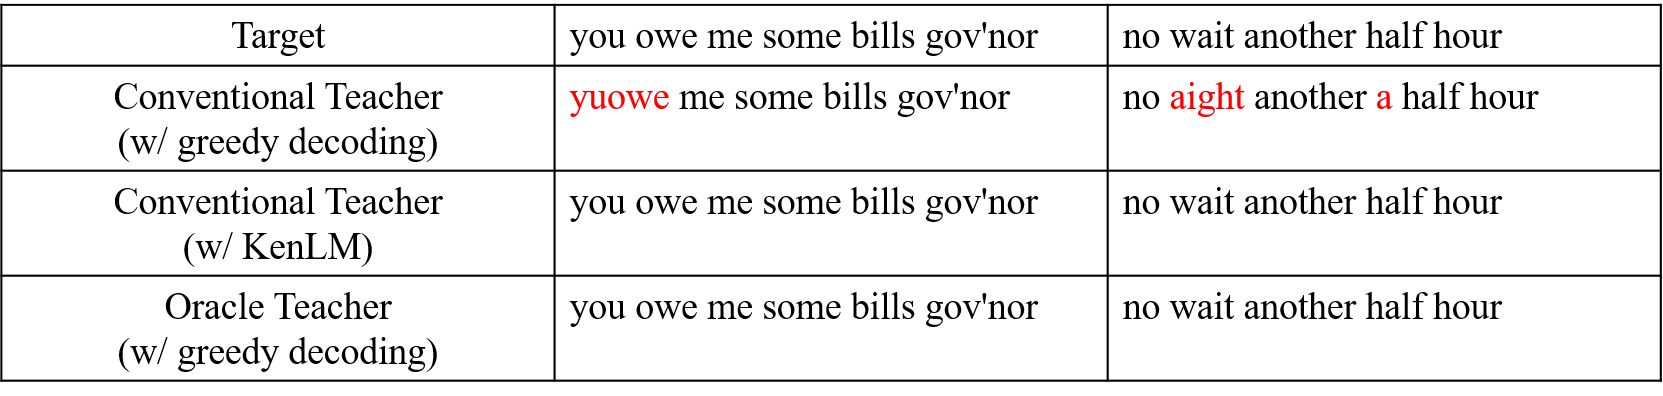
\includegraphics[height=2cm]{case_asr2.png}
	\caption{Recognition example on LibriSpeech test-clean dataset.}
	\label{case_asr2}
\end{figure}

Interestingly, as shown in Fig. \ref{case_asr}, most frames of the conventional teacher had the highest probability for the ``blank" token.
In contrast, the Oracle Teacher had fewer frames that were predicted as ``blank" token. 
This is because the target input $y$ was used as guidance to reduce the candidate scope of the CTC alignment $\pi$.
By using the additional target (text) information, multiple frames of the Oracle Teacher were more likely to be predicted as non-blank character labels rather than the ``blank" during the active speech periods, implying that the representation of the Oracle Teacher could contain much more information about non-blank labels corresponding to the characters (text).



\begin{table}[t]
\centering
{\fontsize{7.3}{8.76}\selectfont
\centering
\caption{WER (\%) performance comparison across CTC-based ASR models on LibriSpeech. The best result of the student is in bold.}
\label{asr_app}
\begin{tabular}{|c|c|c|cc|cc|}
\hline
\multirow{2}{*}{Teacher} & \multirow{2}{*}{Student}     & \multirow{2}{*}{KD method} & \multicolumn{2}{c|}{dev}                            & \multicolumn{2}{c|}{test}                           \\ \cline{4-7} 
                         &                              &                            & \multicolumn{1}{c|}{clean}         & other          & \multicolumn{1}{c|}{clean}         & other          \\ \hline
None                     & \multirow{7}{*}{\makecell{Jasper\\Mini}}                  & None                       & \multicolumn{1}{c|}{8.66}          & 23.28          & \multicolumn{1}{c|}{8.85}          & 24.26          \\ \cline{1-1} \cline{3-7} 
Jasper DR                &  & \multirow{2}{*}{RKD \cite{tutornet:scheme}}                       & \multicolumn{1}{c|}{6.74}          & 19.27          & \multicolumn{1}{c|}{6.77}          & 19.78          \\ \cline{1-1} \cline{4-7} 
Oracle Teacher           &                              &                       & \multicolumn{1}{c|}{\textbf{6.44}} & \textbf{18.36} & \multicolumn{1}{c|}{\textbf{6.43}} & \textbf{18.97} \\ \cline{1-1} \cline{3-7} 
Jasper DR                &                              & \multirow{2}{*}{SKD \cite{tutornet:scheme}}                          & \multicolumn{1}{c|}{7.64}          & 21.36          & \multicolumn{1}{c|}{7.81}          & 22.41          \\ \cline{1-1} \cline{4-7} 
Oracle Teacher           &                              &                       & \multicolumn{1}{c|}{7.57}          & 21.20          & \multicolumn{1}{c|}{7.71}          & 21.71          \\ \cline{1-1} \cline{3-7} 
Jasper DR                &                              & \multirow{2}{*}{FitNets \cite{romero-et-al:scheme}}                      & \multicolumn{1}{c|}{7.05}          & 19.41          & \multicolumn{1}{c|}{7.03}          & 20.41          \\ \cline{1-1} \cline{4-7} 
Oracle Teacher           &                              &                    & \multicolumn{1}{c|}{6.64}          & 18.91          & \multicolumn{1}{c|}{6.67}          & 19.82          \\ \hline
\end{tabular}}
\end{table}

\begin{table*}[t]
% \renewcommand{\tabcolsep}{3.5pt}
\centering
\caption{Computational resource consumption comparison across teacher models.}{% 
{\fontsize{7.3}{8.76}\selectfont
\label{gpu}
% \vspace{-2mm}
\begin{tabular}{|c|c|c|c|c|c|c|c|}
\hline
Task &Training dataset& Teacher model & Params.& GPU & Batch & Times & Epochs \\
\hline
\multirow{2}{*}{ASR}&\multirow{2}{*}{LibriSpeech}&Jasper DR \cite{jasper:scheme}&333 M&8 * 32GB& 256 & - &400 epochs\\
&&\textbf{Oracle Teacher (ours)}&33 M&1 * 12GB& 64 & 22 h &30 epochs\\
\hline
\multirow{2}{*}{ASR}&\multirow{2}{*}{AISHELL-2}&Jasper DR\cite{jasper:scheme} &338 M&8 * 32GB& 128 & - &50 epochs\\
&&\textbf{Oracle Teacher (ours)}&34 M&1 * 12GB& 64 & 118 h &30 epochs\\
\hline
&&Star-Net \cite{starnet:scheme} &49 M&1 * 12GB& 192 &27 h & 300k iter.\\
STR&MJSynth + SynthText&Rosetta \cite{rosetta:scheme}&46 M&1 * 12GB& 192 &27 h& 300k iter.\\
&&\textbf{Oracle Teacher (ours)}& 12 M&1 * 12GB& 192 &10 h& 300k iter.\\
\hline
\end{tabular}%
}}
% \vspace{-5mm}
\end{table*}

In addition, we compared the ASR predictions of the conventional teacher and the Oracle Teacher, as shown in Fig. \ref{case_asr2}.
In Fig. \ref{case_asr2}, the conventional teacher made erroneous predictions with ``yuowe", ``aight", and ``a" using the greedy decoding.
When considering the acoustic (speech) feature only, it is challenging to distinguish some words, such as ``you owe"/``yuowe" and ``wait"/``aight".
The conventional teacher generated an accurate prediction when decoding with the external KenLM that provided additional linguistic information.
However, the proposed Oracle Teacher could produce correct ASR prediction without using the external LM.
This is because the Oracle Teacher leveraged both the source input (speech) and the output label (text) as the teacher model's input.
Unlike the conventional teacher that only considered acoustic features, the Oracle Teacher performed a fusion of acoustic (speech) and linguistic (text) features when generating the prediction.
Since unifying acoustic and linguistic representation learning generally enhances the performance of the speech processing \cite{acours_lin1,acours_lin2,acours_lin3,acours_lin4,acours_lin5}, the Oracle Teacher that considered linguistic information could estimate better CTC prediction, and also its representation was a more supportive knowledge for the ASR student.


\subsection{Performance Comparison with Other KD Methods}
In the previous results, we applied Fitnets \cite{romero-et-al:scheme} as the basic KD method. To further validate the effectiveness of the Oracle Teacher, we used other KD methods for performance comparison.


Firstly, we applied RKD \cite{tutornet:scheme} as the KD method, a recent KD approach in ASR task. It transfers the representation-level knowledge by considering a frame weighting, reflecting which frames were important for KD. 
In addition to the RKD, we adopted SKD \cite{tutornet:scheme} for KD, which effectively transfers the softmax-level knowledge in the CTC framework.
From the results in Table \ref{asr_app}, it is confirmed that Oracle Teacher was more supportive than the conventional Jasper DR teacher in all configurations.
Also, we verified that RKD achieved better improvements than other KD methods, including FitNets and SKD. The best performance was achieved when using the Oracle Teacher with the RKD. We can observe the consistent performance gain of the Oracle Teacher over the conventional teacher for various KD methods.

% \subsubsection{MT} In the case of MT, we used a sequence-level KD (Seq-KD) \cite{mt_kd2}, a widely-used KD in sequence generation tasks, as the additional KD method. The results for IWSLT2016 are shown in Table \ref{mt_app}.
% When using Seq-KD with the Transformer$_{tea}$, the student's performances were even worse than their baselines in many cases, including En-De tst2013, De-En tst2013, En-Fr tst2013, En-Fr tst2014, and Fr-En tst2013.
% However, Seq-KD with the Oracle Teacher improved the student's BLEU performance in all configurations. Moreover, in the case of En-De tst2013, the best performance was yielded when applying the Seq-KD with the Oracle Teacher.
% This implies that the Oracle Teacher was more supportive than the conventional teacher when using not only for the FitNets but also for the Seq-KD.






\subsection{Computational Cost Comparison} 
\label{computational cost section}
In addition to the previous experiments, we proceeded to verify the computational efficiency of the proposed teacher model. Computational resource consumption compared to the conventional teacher models are shown in Table \ref{gpu}.
\subsubsection{Speech Recognition}
Since it is difficult to reproduce the reported WER results of Jasper DR \cite{jasper:scheme} without a large number of resources, we used the checkpoint for LibriSpeech, provided by the OpenSeq2Seq \cite{openseq2seq} toolkit. 
% Also, pre-trained Jasper DR for the Mandarin dataset was provided by the NeMo \cite{nemo:scheme} toolkit.
For LibriSpeech, the pre-trained Jasper DR model required eight 32GB GPUs for 400 epochs with a batch size of 256. Its training time had not been reported previously, either in the paper of Li \textit{et al.} \cite{jasper:scheme} or the toolkit.
In the case of the Oracle Teacher, we trained the model for 30 epochs on a single 12GB GPU, which took about 22 hours ($\approx$ 1 day) to finish the training.
Considering that the reported training of the Quartznet \cite{quartznet:scheme}, which is more computationally efficient than Jasper DR, for 400 epochs took 122 hours ($\approx$ 5 days) with eight 32GB GPUs with a batch size of 256, the Oracle Teacher dramatically reduced the computational cost of the teacher model.
\subsubsection{Scene Text Recognition}
As presented in Table \ref{gpu}, the training of Star-Net \cite{starnet:scheme} took about 27 hours on a single Titan V GPU (12GB) with a total batch size of 192, and the training of Rosetta \cite{rosetta:scheme} required about 27 hours.
Compared to the two conventional models, the training of Oracle Teacher consumed much less training time (10 hours) with the same computational resource.
% , implying that we can obtain the effective teacher with reduced computational cost via the proposed framework.


\subsection{Analysis}
From the previous experimental results, we validate the superiority of the proposed teacher model.
Therefore, it is necessary to test if the model has been correctly trained.
\subsubsection{Visualization of Cross Attention}
\label{visual_cross}

\begin{figure}[t]
% \vspace{-6mm}
\centering
\begin{subfigure}[Oracle Teacher]
	{
		\includegraphics[height=2.2cm]{attention1.jpg}
		\label{attention1}
	}
\end{subfigure}
\begin{subfigure}[Oracle Teacher w/o source]
	{
		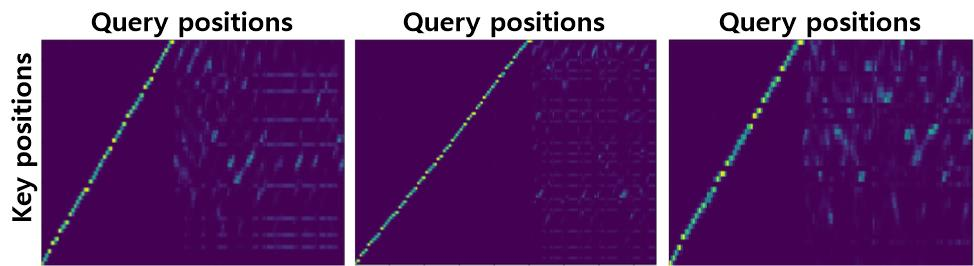
\includegraphics[height=2.2cm]{attention2.jpg}
		\label{attention2}
	}
\end{subfigure}
% \vspace{-2mm}
\caption{Visualization of the attention weights of the Oracle Teacher with and without the source input}
% \vspace{-3mm}
\label{attention}
\end{figure}
We trained another incomplete Oracle Teacher, called Oracle Teacher w/o source. 
The zero arrays, which had the same size of $x$, were treated as the input instead of the source input $x$ during the training. 
% SourceNet only took as input the positional information. 
Then, the Oracle Teacher w/o source only considered the target input $y$ when making a prediction, similar to the aforementioned trivial solution.
In Fig. \ref{attention}, we visualize the cross attention scores
of the decoder for the ASR task, where the x-axis refers to acoustic frames and the y-axis refers to characters.
For the Oracle Teacher w/o source, the attention had almost diagonal alignment along with the key position (text) while ignoring the length of query, as shown in Fig. \ref{attention2}.
In contrast, the Oracle Teacher considered both speech and text alignment in the cross attention, and the attention scores were correctly computed along with the acoustic frames (query), as shown in Fig. \ref{attention1}.
It means that the Oracle Teacher utilized the source $x$ for model training while preventing the trivial solution.
Therefore, we can confirm that the Oracle Teacher, including SourceNet, has been correctly trained.  

\subsubsection{KD with Oracle Teacher w/o source}
In addition to the previous experiments, we proceeded to train the student model with the knowledge of the Oracle Teacher w/o source. However, as we expected, the distilled student failed to converge.
From this additional result, we can verify that the source input $x$ is the necessary factor of the Oracle Teacher, and the proposed Oracle Teacher has been correctly trained.

\subsubsection{Performance of Oracle Teacher} 
\label{per_oracle}
\begin{table}[t]
% \renewcommand{\tabcolsep}{3.5pt}
% \vspace{-5mm}
\centering
\fontsize{7.3}{8.76}\selectfont
\caption{Performance and parameter comparison between the Oracle Teacher and the conventional teacher.}
% \vspace{-2mm}
\begin{tabular}{|c|c|c|cccc|}
\hline
\multirow{3}{*}{Task} & \multirow{3}{*}{Model} & \multirow{3}{*}{Param.} & \multicolumn{4}{c|}{WER (\%)} \\ \cline{4-7} 
 &  &  & \multicolumn{2}{c|}{dev} & \multicolumn{2}{c|}{test} \\ \cline{4-7} 
 &  &  & \multicolumn{1}{c|}{clean} & \multicolumn{1}{c|}{other} & \multicolumn{1}{c|}{clean} & other \\ \hline
\multirow{2}{*}{ASR} & Jasper DR \cite{jasper:scheme}& 333 M & \multicolumn{1}{c|}{3.61} & \multicolumn{1}{c|}{11.37} & \multicolumn{1}{c|}{\textbf{3.77}} & 11.08 \\ \cline{2-7} 
 & Oracle Teacher & 33 M & \multicolumn{1}{c|}{\textbf{2.87}} & \multicolumn{1}{c|}{\textbf{3.10}} & \multicolumn{1}{c|}{4.03} & \textbf{3.29} \\ \hline
\end{tabular}
\label{oracle_perform}
% \vspace{-3mm}
\end{table}
We also evaluated the performance of the Oracle Teacher itself compared to the conventional teachers, as shown in Table \ref{oracle_perform}.
If the Oracle Teacher copies the target input $y$ without utilizing the source input $x$, the performance of the Oracle Teacher should be perfect.
We measured WER (\%) results on LibriSpeech.
% In the case of MT, the teacher forcing and the greedy decoding were applied during the evaluation since we generally use teacher forcing when extracting the knowledge from an autoregressive teacher model.
The results show that the performance of the Oracle Teacher was more effective than that of the conventional teacher model, which seemed reasonable because the Oracle Teacher was trained with the guidance of $y$.
Meanwhile, the predictions of the Oracle Teacher were not the same as each ground truth. 
This implies that the Oracle teacher's output did not simply copy the target input $y$, and the information from a properly-trained SourceNet was utilized to generate the prediction.
Compared to the ``clean" datasets, the difference of WER was huge in ``other" sets.
Since the ``other" dataset represents a noisy dataset, the conventional ASR model (Jasper DR) showed low performance for the ``other" dataset. However, the Oracle Teacher could result in high performance for the noisy dataset since it used text information from the target.
This indicates that the Oracle Teacher could be a noisy robust teacher with small parameters.
From the results, we can verify that the Oracle Teacher provided more accurate and better guidance to the student than the conventional ASR teacher model.

\section{Discussion} 
This work offered a powerful but efficient KD method in the context of CTC-based sequence learning tasks. 
However, the use of output labels as the additional input for the teacher model could limit its usage on unsupervised data. 
One possible way to apply the Oracle Teacher in the unsupervised setting is leveraging the prediction as the model's input, like \cite{target1,imputer,mask-ctc}.
However, in Section \ref{case_sec}, it is confirmed that the Oracle Teacher gave accurate CTC alignment by utilizing the ground-truth labels as the additional input.
Since the target input was used as guidance to reduce the candidate scope of the alignment, using the erroneous prediction as the additional input might significantly degrade the performance of the Oracle Teacher.
Extending the proposed framework further, using the Oracle Teacher on unsupervised data is our future work.

\section{Conclusions}
We introduced a novel teacher for CTC-based sequence models, namely Oracle Teacher, that leverages the output labels as the additional input to the model.
Through a number of experiments, we confirmed that the student distilled from the Oracle Teacher performed better compared to the one distilled from the conventional teacher.
Furthermore, our framework significantly reduced the computational cost of the teacher model in terms of the training time and required GPU resources.
As the effective teacher can be trained with a reduced computational cost, the Oracle Teacher can be a new breakthrough in KD.
We expect the application of the Oracle Teacher in various tasks, such as regression, ranking, etc., in the future.


% \section*{Acknowledgement}
% This work was supported by Samsung Electronics Co., Ltd. (IO201211-08075-01)

\ifCLASSOPTIONcaptionsoff
  \newpage
\fi


\bibliographystyle{unsrt}
\bibliography{Trans.bib}

\end{document}


